\section{How LLVM handles debug information\label{sec:llvm-dbg}}

\subsection{Metadata classes}
\subsection{Transformation passes guidelines}
As we've seen in section \ref{sec:llvm-passes}, during the compilation a module may undergo some changes: instructions may be removed, moved, merged together, and replaced with new instructions, all in order to improve the performances of the resulting program. \par 
This transformations have the side effect of obfuscating the correspondence between source code and binary code: before the optimization occurs, debug information provide a very clear, one to many relation between source location and LLVM-IR instructions. But as the module progresses into the optimization pipeline, it becomes more and more difficult to maintain this relation. \par
In general it is not possible to map unambiguously source locations to optimized code, but the LLVM project provides a set of guidelines that specify how to correctly update debug info when implementing transformation passes \cite{llvm-guidelines}. \newline
Here we provide a short summary of such guidelines \footnote{Provided at a speech and the 2020 LLVM Conference by Adrian Pranti and Vedant Kumar}, highlighting some behaviors that, even when following them, lead to a loss of information regarding source-binary mapping. This behaviors are not bug or mistakes of the people who provided the guidelines, but are instead related to the fact that they want to provide a debugging experience as close as possible to the one that a user would have while debugging the unoptimized code. \par 
The guiding principles for a developer that wants to update debug info are the following:
\begin{enumerate}
\item Do not provide misleading information: a developer should not speculate, and providing no information is better than providing wrong information that may lead a developer to wrong considerations about the behavior of his program.
\item Provide as much information as possible: when it's not misleading, information should be preserved. 
\end{enumerate}
In order to achieve this, when choosing what do to with the debug information of a given instruction, a developer has three alternatives:
\begin{itemize}
\item Preserve the original location.
\item Merge two locations: two debug locations can be merged together. Locations merge is performed by computing the intersection of the two locations: the resulting location will contain only the information that the original two had in common.
\item Delete the location.
\end{itemize}
Locations can be safely preserved when the modified instruction either remains in the same basic block, or its basic block is folded into a predecessor that branches unconditionally. For instance, an optimization the replaces the instruction {\fontfamily{qcr}\selectfont add x x} with a binary shift to the left ({\fontfamily{qcr}\selectfont shl x 1}) can safely keep the location of the original add. \par 
Location should be merged when two instructions are replaced with a new instruction. An example of that is figure \ref{fig:merge}, in which the two stores can be merged into a new one, inserted in the exit basic block: the new instruction effectively replaces the original two, and therefore its location will be the merged location of the old ones. \par
\begin{figure}
\centering
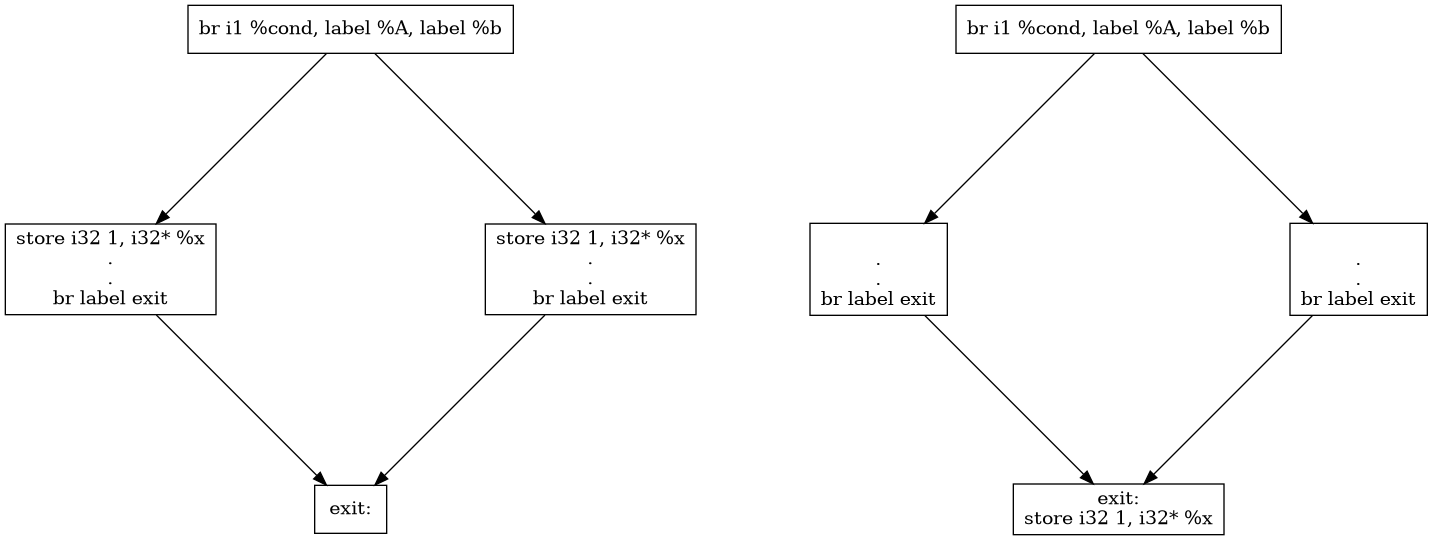
\includegraphics[scale=0.3]{chapter-2/merge.png}
\caption{Example of optimization with merged debug location}
\label{fig:merge}
\end{figure}

\section{Energy consumption estimation}

